
%(BEGIN_QUESTION)
% Copyright 2011, Tony R. Kuphaldt, released under the Creative Commons Attribution License (v 1.0)
% This means you may do almost anything with this work of mine, so long as you give me proper credit

Tegn inn nødvendige koblinger for å koble en solenoid og en relespole til h.h.v. inngang \texttt{Qx.2} og \texttt{Qx.4} på en Siemens SM322 DO modul(model 6ES7322-1FH00-0AA0). Begge spolene har en normert spenning på 230VAC. Det interne skjemaet for den første utgangen vises som referanse. Her vises hvordan en TRIAC blir brukt som bryter for å gi spenning på de digitale utgangene. 

$$\includegraphics[width=15.5cm]{i04246x01.eps}$$

Forklar også tretsen inni modulen virker, følge effektkretsen igjennom modulen. 

\vskip 20pt \vbox{\hrule \hbox{\strut \vrule{} {\bf Suggestions for Socratic discussion} \vrule} \hrule}

\begin{itemize}
\item{} What function does the ``SF'' LED perform, and what makes it turn on?
\end{itemize}

\underbar{file i04246}
%(END_QUESTION)





%(BEGIN_ANSWER)

$$\includegraphics[width=15.5cm]{i04246x02.eps}$$

%(END_ANSWER)





%(BEGIN_NOTES)


%INDEX% PLC, I/O: discrete I/O device wiring

%(END_NOTES)


